\documentclass{article}

\usepackage{listings}
\usepackage{xcolor}
\usepackage{caption}
\usepackage[a4paper, total={6in, 10in}]{geometry}
\usepackage[utf8x]{inputenc}
\usepackage[framemethod=tikz]{mdframed}

\lstset{
  language=C,               
  numbers=left,             
  stepnumber=1,             
  numbersep=10pt,           
  backgroundcolor=\color{white},
  showspaces=false,             
  showtabs=false,               
  tabsize=2,                    
  captionpos=b,                 
  breaklines=true,              
  breakatwhitespace=true,       
  belowcaptionskip=1\baselineskip,
  breaklines=true,
  xleftmargin=\parindent,
  showstringspaces=false,
  basicstyle=\footnotesize\ttfamily,
  keywordstyle=\bfseries\color{blue!40!black},
  commentstyle=\itshape\color{green!40!black},
  stringstyle=\color{orange},
}

\newcommand\mylstcaption{}

\mdfdefinestyle{mymdstyle}{
hidealllines=true,
middleextra={
  \node[anchor=west] at (O|-P)
    {\lstlistingname~\thelstlisting\  (Cont.):~\mylstcaption};},
secondextra={
  \node[anchor=west] at (O|-P)
    {\lstlistingname~\thelstlisting\  (Cont.):~\mylstcaption};},
splittopskip=2\baselineskip
}

\surroundwithmdframed[style=mymdstyle]{lstlisting}
\newmdenv[style=mymdstyle]{mdlisting}

\begin{document}
\section{Part A: Writing a Cache Simulator}
\paragraph{Solution}
The source code of data cache simulator with least recently used (LRU) cache level policy
is presented on listing \ref{lst:c1}.
\renewcommand\mylstcaption{csim.c}
\begin{mdlisting}
  \lstinputlisting[caption=\mylstcaption, label=lst:c1]{../csim.c}
\end{mdlisting}
The program was run against the reference simulator.
The screenshot of the test benchmark run is presented on figure \ref{fig:test-run}.
\begin{figure}[h]
  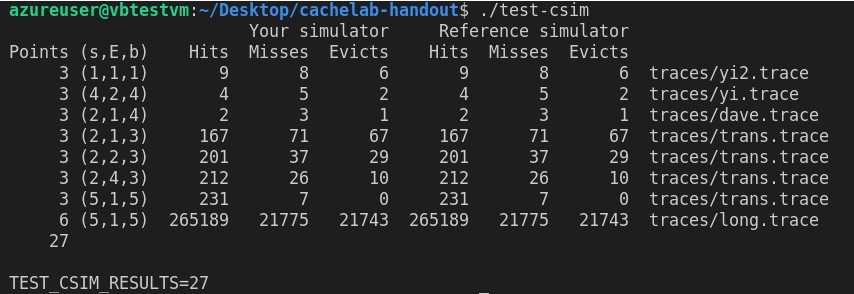
\includegraphics[width=0.6\textwidth]{test_results.jpg}
  \centering
  \caption{Benchmark results}
  \label{fig:test-run}
\end{figure}
\section{Part B: Optimizing Matrix Transpose}
The solution includes three different transpose functions for matrices with sizes:
\begin{itemize}
  \item $ 32 \times 32 $
  \item $ 64 \times 64 $
  \item $ 32 \times 32 $
\end{itemize}
The full source code of \textsf{trans.c} is show on listing \ref{lst:c2}.
\renewcommand\mylstcaption{csim.c}
\begin{mdlisting}
  \lstinputlisting[caption=\mylstcaption, label=lst:c2]{../trans.c}
\end{mdlisting}
The screenshot of the full lab benchmark run is presented on figure \ref{fig:final-run}.
\begin{figure}[h]
  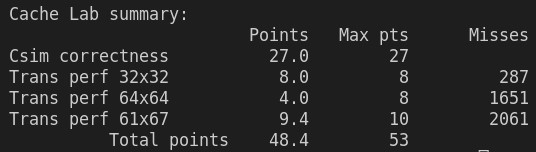
\includegraphics[width=0.6\textwidth]{final_results.jpg}
  \centering
  \caption{Final lab results}
  \label{fig:final-run}
\end{figure}
\end{document}